\section{Nonlinear signal Analysis}



\begin{figure}[!htbp]
\minipage{.5\textwidth}%
\centering
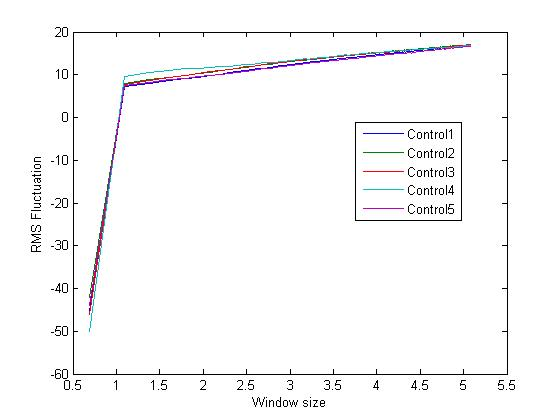
\includegraphics[width=.8\textwidth]{E1.jpg}
\subcaption{DFA result of the control data set}\label{figa}
\endminipage\hfill
\minipage{.5\textwidth}%
\centering
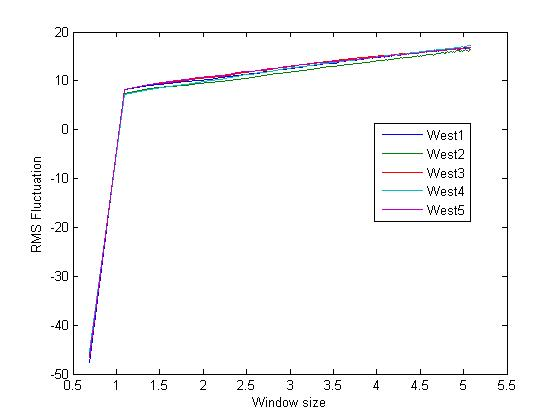
\includegraphics[width=.8\textwidth]{E2.jpg}
\subcaption{DFA result of the west data set}\label{figb}
\endminipage\hfill
\caption{Detrended fluctation analysis plots of the two data set}
\end{figure}


\begin{table}[!htbp]
\centering
\caption{}\label{c1}
\begin{tabular}{ c c c c c c c c} 
\hline
$Control$&$1$&$2$&$3$&$4$&$5$&$\mu$&$\sigma$\\
\hline
$FD $&$1.7438$&$1.7298$&$1.7707$&$1.7208$&$1.7173$&$ 1.7365$&$ 4.7074e-04$\\
$1/f$&$-1.3486$&$-1.0308$&$-1.0754$&$-1.0624$&$-1.5117$&$-1.2058$&$ 0.0455$\\
$LE$&$0.0826$&$0.3860$&$0.2120$&$0.0825$&$0.0944$&$0.1938$&$0.0198$\\
$SampEnResults$&$2.3058$&$2.0164$&$2.0987$&$1.8646$&$2.1077$&$2.0786$&$0.0256$\\
&$0.6178$&$0.6472$&$0.7670$&$0.4271$&$0.5736$&$0.6065$&$0.0152$\\
\hline 
\end{tabular}
\end{table}

\begin{table}[!htbp]
\centering
\caption{}\label{c2}
\begin{tabular}{ c c c c c c c c} 
\hline
$West$&$1$&$2$&$3$&$4$&$5$&$\mu$&$\sigma$\\
\hline
$FD$&$1.7448$&$1.5999$&$1.7198$&$1.7501$&$1.7059$&$ 1.7041$&$ 0.0037$\\
$1/f$&$-1.0898$&$-1.5659$&$-1.0138$&$-1.3829$&$-1.1288$&$-1.2362$&$ 0.0532$\\
$LE$&$0.1217$&$0.0878$&$0.2797$&$0.0807$&$0.3043$&$0.3222$&$0.0829$\\  
$SampEnResults$&$2.0307$&$2.2033$&$2.1825$&$2.1837$&$2.2467$&$2.1694$&$0.0067$\\
&$1.0327$&$0.6303$&$0.8739$&$0.5220$&$0.6609$&$ 0.7440$&$0.0423$\\
\hline 
\end{tabular}
\end{table}

Non linear analysis of heart rate variability (HRV) aims consistent inference the underlying phenomenon associated with the signal. 
The analysis is divided into two main set of the approaches. 

Starting with the scaling behavior of the non-linearity fractal dimension (FD) is capable of evaluating the complexity degree associated with the signal. This is computed via the of velocity that measurement increases of decreases as the scale tends to increases or decreases. Generally speaking, for abnormal subjects the rhythmic variation tends to decreases consequently FD in this case will be lower than normal subjects. Comparing the two data set in the \textbf{\textit{Control}} case in table \ref{c1} the values of the are fairly high, and there is no variation among the entities. In comparison to the \textbf{\textit{West}} the FD values are on average lower. The variation is slightly higher in this case where in addition the second measurement tends to have a significantly lower value implying some anomalies associated with this patient. Statistically speaking, the west data set on average tends to have less rhythmic heart rate table \ref{c2}.

\textbf{1/f} slope is another important characterisation of the HRV. The smoothness of the time series what the slope values claim to indicate. The values of abnormalities tends to be slightly lower compare to normal HR. In the \textbf{\textit{Control}} data set this values on average tend to be lower compare to the \textbf{\textit{West}} data set although the difference is relatively small. Regarding the variation of this value in the \textbf{\textit{West}} dataset it tends to be bigger. In both group of measurements there are some samples with significantly lower value of slope compare to the mean. In the \textbf{\textit{Control}} case the second, third and fourth sample have a fairly small value. Whereas on the \textbf{\textit{West}} data set the first and the third sample has dramatic low value. 

The other set of measurements consist on the chaos complexity of the system. This methods are mainly based on the chaos theory.

Herein the Lyapunov exponent is the first to be explored. Geometrically speaking  its values represent the divergence of respective trajectories from their initial position. Consequently slowly varying HR, LE is small meaning that the intensity of the chaotic system is low as well. \textbf{\textit{Control}} likewise the average is significantly smaller compare to the \textbf{\textit{West}} data set. Variance is not a of an important as compare to mean however the \textbf{\textit{West}} data set samples vary more. 

Moving on to the sample entropy. It measures statistically the complexity and regularity of the time-series. Its values are small when the HRV runs under same abnormalities and theoretically should be big when the HRV is normal. Mean value is however smaller in the \textbf{\textit{Control}} and therefore inferring some abnormalities compare to the \textbf{\textit{West}}.    
  
Regarding DFA results for low window size tends to be higher in the control case tends to be higher than one. On the other hand the Control case it higher than the West set comparing respective individuate and therefore on average. Translated into variability the West case on average has a higher variation compare to the Control set in figure \ref{figa} and \ref{figb}. Further more from the table \ref{a2} and \ref{a1} the slopes are computed from the DFA plots are outlined into the both tables. Speaking about the health, Control set has a higher variability compare to the West which is the main indication of the DFA from higher slope value.  
    
    




\begin{table}[!htbp]
\centering
\caption{Slope of the second part of line in DFA plots}\label{a2}
\begin{tabular}{ c c c c c c c c} 
\hline
&$1$&$2$&$3$&$4$&$5$&$\mu$\\
\hline
$Control$&$31.4300$&$ 4.8353$&$4.8058$&$15.0472$&$21.1844$&$6.9868$\\
$West$&$6.9512$&$ 3.7947$&$0.7843$&$ 0.6201$&$13.9351$&$5.2171$\\
\hline 
\end{tabular}
\end{table}





\begin{table}[!htbp]
\centering
\caption{Slope of the first part of line in DFA plots}\label{a1}
\begin{tabular}{ c c c c c c c c} 
\hline
&$1$&$2$&$3$&$4$&$5$&$\mu$\\
\hline
$Control$&$129.5984$&$123.5662$&$132.5211$&$147.3374$&$127.0359$&$132.0118$\\
$West$&$137.6878$&$132.0872$&$135.5602$&$129.5709$&$135.0323$&$133.9877$\\
\hline 
\end{tabular}
\end{table}



\begin{figure}[!htbp]
\minipage{.5\textwidth}%
\centering
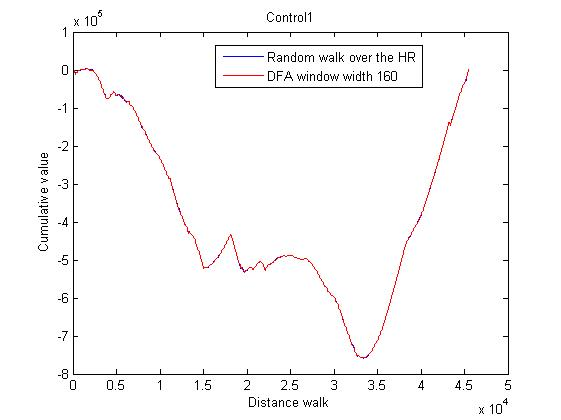
\includegraphics[width=.7\textwidth]{E3.jpg}\\
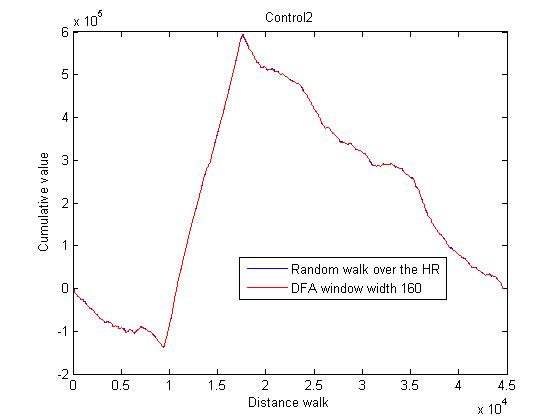
\includegraphics[width=.7\textwidth]{E4.jpg}\\
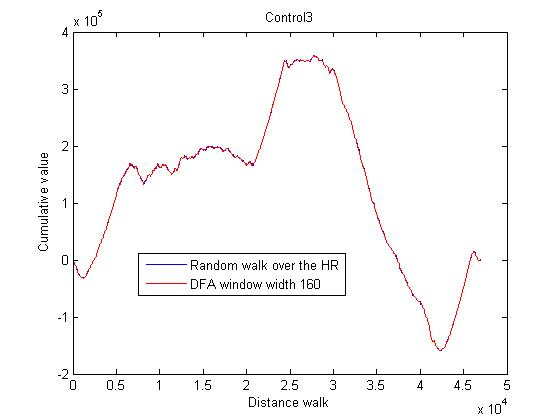
\includegraphics[width=.7\textwidth]{E5.jpg}\\
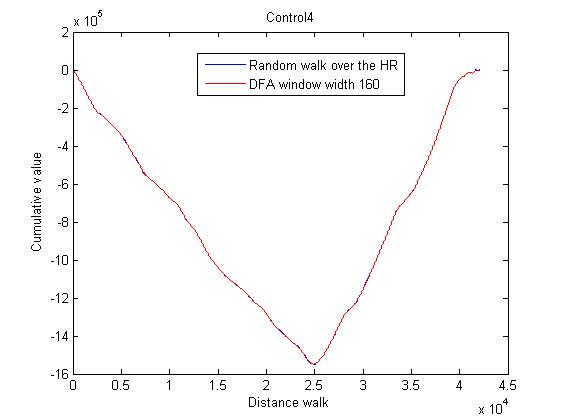
\includegraphics[width=.7\textwidth]{E6.jpg}\\
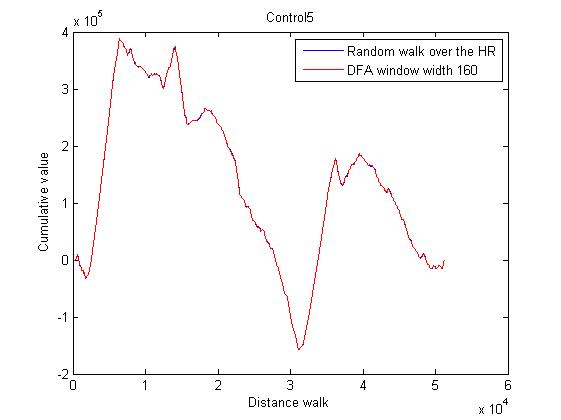
\includegraphics[width=.7\textwidth]{E7.jpg}\\
\subcaption{}
\endminipage\hfill
\minipage{.5\textwidth}%
\centering
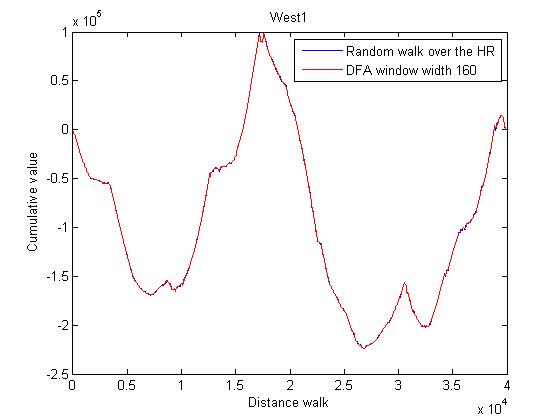
\includegraphics[width=.7\textwidth]{E8.jpg}\\
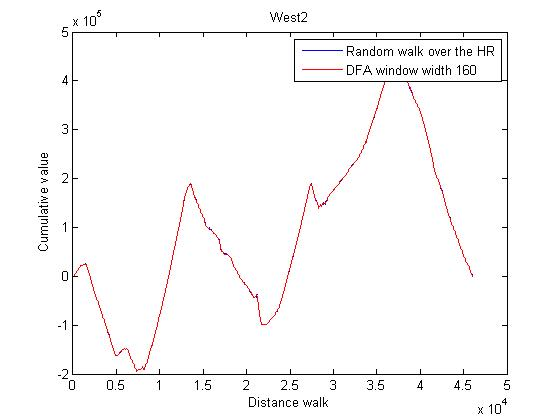
\includegraphics[width=.7\textwidth]{E9.jpg}\\
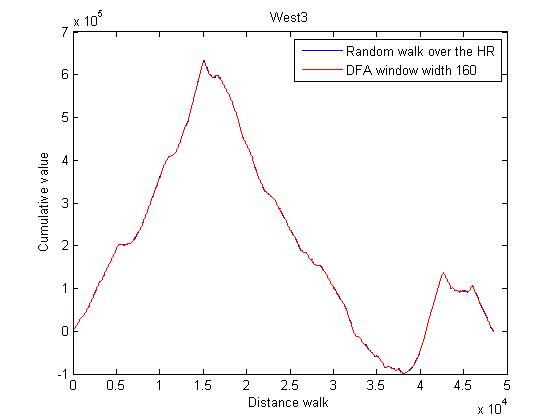
\includegraphics[width=.7\textwidth]{E10.jpg}\\
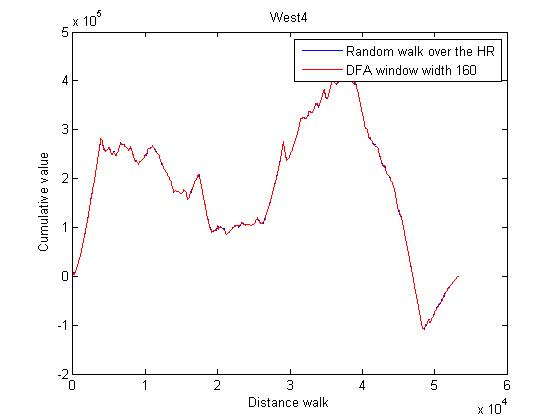
\includegraphics[width=.7\textwidth]{E11.jpg}\\
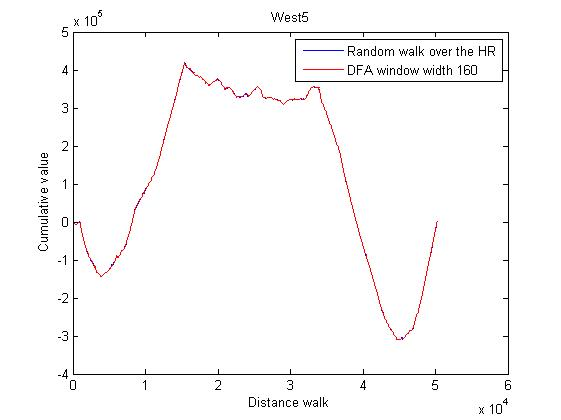
\includegraphics[width=.7\textwidth]{E12.jpg}\\
\subcaption{}
\endminipage\hfill
\caption{DFA result for both of the groups}
\end{figure}



